% PARTE 2 DE 3: EJEMPLOS RESUELTOS, EJERCICIOS INVERSOS Y SOLUCIONES
% Guía de Identidades Trigonométricas - Grado 10

\section{Ejemplos Resueltos}

Ahora vamos a poner en práctica todas las identidades trigonométricas que hemos aprendido. Cada ejemplo está completamente desarrollado paso a paso para que entiendas perfectamente el proceso. ¡Vamos a dominar estas identidades!

\begin{ejemplo}[title=Ejemplo 1: Verificar una identidad pitagórica básica]
Verifica que la siguiente expresión es una identidad verdadera para todo valor de $\theta$ donde las funciones están definidas:
\[
\sec^2\theta - \tan^2\theta = 1
\]

\vspace{0.3cm}
\textbf{Solución:}

\textbf{Paso 1:} Expresar las funciones en términos de seno y coseno.

Recordemos que $\sec\theta = \frac{1}{\cos\theta}$ y $\tan\theta = \frac{\sin\theta}{\cos\theta}$

\textbf{Paso 2:} Sustituir en el lado izquierdo de la identidad.
\begin{align*}
\sec^2\theta - \tan^2\theta &= \left(\frac{1}{\cos\theta}\right)^2 - \left(\frac{\sin\theta}{\cos\theta}\right)^2 \\[0.3cm]
&= \frac{1}{\cos^2\theta} - \frac{\sin^2\theta}{\cos^2\theta}
\end{align*}

\textbf{Paso 3:} Encontrar un denominador común y simplificar.
\begin{align*}
\frac{1}{\cos^2\theta} - \frac{\sin^2\theta}{\cos^2\theta} &= \frac{1 - \sin^2\theta}{\cos^2\theta}
\end{align*}

\textbf{Paso 4:} Aplicar la identidad pitagórica fundamental.

Sabemos que $\sin^2\theta + \cos^2\theta = 1$, por lo tanto: $\cos^2\theta = 1 - \sin^2\theta$

\textbf{Paso 5:} Sustituir y simplificar.
\begin{align*}
\frac{1 - \sin^2\theta}{\cos^2\theta} &= \frac{\cos^2\theta}{\cos^2\theta} \\[0.2cm]
&= 1 \quad \checkmark
\end{align*}

\textbf{Paso 6:} Verificación gráfica usando el círculo unitario.

\begin{center}
\begin{tikzpicture}[scale=3]
    \begin{axis}[
        axis lines = center,
        xlabel = {$x$},
        ylabel = {$y$},
        xmin=-1.5, xmax=1.5,
        ymin=-1.5, ymax=1.5,
        axis equal,
        grid=major,
        width=10cm,
        height=10cm,
    ]
    % Círculo unitario
    \addplot[domain=0:360, samples=100, maincolor, very thick]
        ({cos(x)}, {sin(x)});

    % Punto en el círculo para ángulo de 45 grados
    \addplot[only marks, mark=*, mark size=3pt, maincolor]
        coordinates {({cos(45)}, {sin(45)})};

    % Radio
    \addplot[accentcolor, thick, -{Latex}]
        coordinates {(0,0) ({cos(45)}, {sin(45)})};

    % Proyecciones
    \addplot[dashed, gray]
        coordinates {({cos(45)}, 0) ({cos(45)}, {sin(45)})};
    \addplot[dashed, gray]
        coordinates {(0, {sin(45)}) ({cos(45)}, {sin(45)})};

    % Etiquetas
    \node at (axis cs:0.9, 0.9) {$P(\cos\theta, \sin\theta)$};
    \node at (axis cs:0.5, -0.15) {$\cos\theta$};
    \node at (axis cs:-0.2, 0.5) {$\sin\theta$};
    \end{axis}
\end{tikzpicture}
\end{center}

\textbf{Respuesta final:} $\boxed{\text{Identidad verificada: } \sec^2\theta - \tan^2\theta = 1}$
\end{ejemplo}

\begin{ejemplo}[title=Ejemplo 2: Simplificar expresión con identidades recíprocas]
Simplifica la siguiente expresión trigonométrica usando identidades recíprocas:
\[
\frac{\sin\theta \cdot \csc\theta + \cos\theta \cdot \sec\theta}{\tan\theta \cdot \cot\theta}
\]

\vspace{0.3cm}
\textbf{Solución:}

\textbf{Paso 1:} Aplicar las identidades recíprocas fundamentales.

Recordemos que:
\begin{itemize}
    \item $\sin\theta \cdot \csc\theta = 1$
    \item $\cos\theta \cdot \sec\theta = 1$
    \item $\tan\theta \cdot \cot\theta = 1$
\end{itemize}

\textbf{Paso 2:} Sustituir estas identidades en la expresión.
\begin{align*}
\frac{\sin\theta \cdot \csc\theta + \cos\theta \cdot \sec\theta}{\tan\theta \cdot \cot\theta} &= \frac{1 + 1}{1} \\[0.3cm]
&= \frac{2}{1} \\[0.3cm]
&= 2
\end{align*}

\textbf{Paso 3:} Verificación desarrollando las funciones recíprocas.

Vamos a verificar expandiendo cada función:
\begin{align*}
\frac{\sin\theta \cdot \frac{1}{\sin\theta} + \cos\theta \cdot \frac{1}{\cos\theta}}{\frac{\sin\theta}{\cos\theta} \cdot \frac{\cos\theta}{\sin\theta}} &= \frac{\frac{\sin\theta}{\sin\theta} + \frac{\cos\theta}{\cos\theta}}{\frac{\sin\theta \cdot \cos\theta}{\cos\theta \cdot \sin\theta}} \\[0.3cm]
&= \frac{1 + 1}{1} = 2 \quad \checkmark
\end{align*}

\textbf{Paso 4:} Interpretación geométrica.

Esta simplificación nos dice que no importa el valor del ángulo $\theta$ (siempre que las funciones estén definidas), la expresión siempre vale 2. ¡Es una constante!

\textbf{Respuesta final:} $\boxed{2}$
\end{ejemplo}

\begin{ejemplo}[title=Ejemplo 3: Expresar seno en términos de coseno]
Si $\cos\theta = \frac{3}{5}$ y $\theta$ está en el cuarto cuadrante, expresa todas las demás funciones trigonométricas en términos del coseno dado.

\vspace{0.3cm}
\textbf{Solución:}

\textbf{Paso 1:} Encontrar $\sin\theta$ usando la identidad pitagórica.

De $\sin^2\theta + \cos^2\theta = 1$:
\begin{align*}
\sin^2\theta &= 1 - \cos^2\theta \\
&= 1 - \left(\frac{3}{5}\right)^2 \\
&= 1 - \frac{9}{25} \\
&= \frac{25 - 9}{25} = \frac{16}{25}
\end{align*}

\textbf{Paso 2:} Determinar el signo de $\sin\theta$.

Como $\theta$ está en el cuarto cuadrante, sabemos que $\sin\theta < 0$.

Por lo tanto: $\sin\theta = -\sqrt{\frac{16}{25}} = -\frac{4}{5}$

\textbf{Paso 3:} Calcular la tangente.
\[
\tan\theta = \frac{\sin\theta}{\cos\theta} = \frac{-4/5}{3/5} = -\frac{4}{5} \cdot \frac{5}{3} = -\frac{4}{3}
\]

\textbf{Paso 4:} Calcular las funciones recíprocas.
\begin{align*}
\csc\theta &= \frac{1}{\sin\theta} = \frac{1}{-4/5} = -\frac{5}{4} \\[0.3cm]
\sec\theta &= \frac{1}{\cos\theta} = \frac{1}{3/5} = \frac{5}{3} \\[0.3cm]
\cot\theta &= \frac{1}{\tan\theta} = \frac{1}{-4/3} = -\frac{3}{4}
\end{align*}

\textbf{Paso 5:} Verificación usando el teorema de Pitágoras.

En un triángulo rectángulo con hipotenusa 5, cateto adyacente 3 y cateto opuesto 4:
\[
3^2 + 4^2 = 9 + 16 = 25 = 5^2 \quad \checkmark
\]

\textbf{Paso 6:} Representación en el círculo unitario.

\begin{center}
\begin{tikzpicture}[scale=2.5]
    \begin{axis}[
        axis lines = center,
        xlabel = {$x$},
        ylabel = {$y$},
        xmin=-1.2, xmax=1.2,
        ymin=-1.2, ymax=1.2,
        axis equal,
        grid=major,
        width=8cm,
        height=8cm,
    ]
    % Círculo unitario
    \addplot[domain=0:360, samples=100, maincolor, thick]
        ({cos(x)}, {sin(x)});

    % Punto en el cuarto cuadrante
    \addplot[only marks, mark=*, mark size=3pt, red]
        coordinates {(0.6, -0.8)};

    % Radio
    \addplot[red, thick, -{Latex}]
        coordinates {(0,0) (0.6, -0.8)};

    % Proyecciones
    \addplot[dashed, gray]
        coordinates {(0.6, 0) (0.6, -0.8)};
    \addplot[dashed, gray]
        coordinates {(0, -0.8) (0.6, -0.8)};

    % Etiquetas
    \node at (axis cs:0.85, -0.85) {$(\frac{3}{5}, -\frac{4}{5})$};
    \node at (axis cs:0.3, -0.15) {$\theta$};
    \end{axis}
\end{tikzpicture}
\end{center}

\textbf{Respuesta final:}
\[
\boxed{
\begin{aligned}
\sin\theta &= -\frac{4}{5}, \quad \tan\theta = -\frac{4}{3}, \quad \csc\theta = -\frac{5}{4} \\
\sec\theta &= \frac{5}{3}, \quad \cot\theta = -\frac{3}{4}
\end{aligned}
}
\]
\end{ejemplo}

\begin{ejemplo}[title=Ejemplo 4: Demostrar una identidad trigonométrica]
Demuestra la siguiente identidad trigonométrica:
\[
\frac{1 + \tan^2\theta}{\sec\theta} = \sec\theta
\]

\vspace{0.3cm}
\textbf{Solución:}

\textbf{Paso 1:} Trabajar con el lado izquierdo de la identidad.

Vamos a transformar el lado izquierdo hasta llegar al lado derecho.

\textbf{Paso 2:} Aplicar la identidad pitagórica $1 + \tan^2\theta = \sec^2\theta$.

\begin{align*}
\frac{1 + \tan^2\theta}{\sec\theta} &= \frac{\sec^2\theta}{\sec\theta}
\end{align*}

\textbf{Paso 3:} Simplificar la fracción.
\begin{align*}
\frac{\sec^2\theta}{\sec\theta} &= \sec\theta \cdot \frac{\sec\theta}{\sec\theta} \\
&= \sec\theta \cdot 1 \\
&= \sec\theta \quad \checkmark
\end{align*}

\textbf{Paso 4:} Verificación alternativa usando definiciones básicas.

Expresemos todo en términos de seno y coseno:
\begin{align*}
\text{Lado izquierdo} &= \frac{1 + \tan^2\theta}{\sec\theta} \\
&= \frac{1 + \frac{\sin^2\theta}{\cos^2\theta}}{\frac{1}{\cos\theta}} \\
&= \frac{\frac{\cos^2\theta + \sin^2\theta}{\cos^2\theta}}{\frac{1}{\cos\theta}}
\end{align*}

\textbf{Paso 5:} Aplicar la identidad fundamental $\sin^2\theta + \cos^2\theta = 1$.
\begin{align*}
&= \frac{\frac{1}{\cos^2\theta}}{\frac{1}{\cos\theta}} \\
&= \frac{1}{\cos^2\theta} \cdot \frac{\cos\theta}{1} \\
&= \frac{1}{\cos\theta} = \sec\theta \quad \checkmark
\end{align*}

\textbf{Paso 6:} Verificación numérica con $\theta = 60°$.

Para $\theta = 60°$: $\cos 60° = \frac{1}{2}$, $\sin 60° = \frac{\sqrt{3}}{2}$

$\tan 60° = \sqrt{3}$, $\sec 60° = 2$

Lado izquierdo: $\frac{1 + (\sqrt{3})^2}{2} = \frac{1 + 3}{2} = \frac{4}{2} = 2 = \sec 60°$ ✓

\textbf{Respuesta final:} $\boxed{\text{Identidad demostrada: } \frac{1 + \tan^2\theta}{\sec\theta} = \sec\theta}$
\end{ejemplo}

\begin{ejemplo}[title=Ejemplo 5: Aplicar identidad de suma de ángulos]
Encuentra el valor exacto de $\sin 75°$ usando la identidad de suma de ángulos.

\vspace{0.3cm}
\textbf{Solución:}

\textbf{Paso 1:} Expresar $75°$ como suma de ángulos conocidos.

$75° = 45° + 30°$

\textbf{Paso 2:} Aplicar la identidad de suma para el seno.

La identidad de suma es: $\sin(\alpha + \beta) = \sin\alpha \cos\beta + \cos\alpha \sin\beta$

\textbf{Paso 3:} Sustituir $\alpha = 45°$ y $\beta = 30°$.
\begin{align*}
\sin 75° &= \sin(45° + 30°) \\
&= \sin 45° \cos 30° + \cos 45° \sin 30°
\end{align*}

\textbf{Paso 4:} Recordar los valores exactos de las funciones.
\begin{itemize}
    \item $\sin 45° = \frac{\sqrt{2}}{2}$, $\cos 45° = \frac{\sqrt{2}}{2}$
    \item $\sin 30° = \frac{1}{2}$, $\cos 30° = \frac{\sqrt{3}}{2}$
\end{itemize}

\textbf{Paso 5:} Sustituir y calcular.
\begin{align*}
\sin 75° &= \frac{\sqrt{2}}{2} \cdot \frac{\sqrt{3}}{2} + \frac{\sqrt{2}}{2} \cdot \frac{1}{2} \\[0.3cm]
&= \frac{\sqrt{6}}{4} + \frac{\sqrt{2}}{4} \\[0.3cm]
&= \frac{\sqrt{6} + \sqrt{2}}{4}
\end{align*}

\textbf{Paso 6:} Verificación usando la identidad de suma para el coseno.

$\cos 75° = \cos(45° + 30°) = \cos 45° \cos 30° - \sin 45° \sin 30°$

$= \frac{\sqrt{2}}{2} \cdot \frac{\sqrt{3}}{2} - \frac{\sqrt{2}}{2} \cdot \frac{1}{2} = \frac{\sqrt{6} - \sqrt{2}}{4}$

Verificamos que $\sin^2 75° + \cos^2 75° = 1$:
\[
\left(\frac{\sqrt{6} + \sqrt{2}}{4}\right)^2 + \left(\frac{\sqrt{6} - \sqrt{2}}{4}\right)^2 = \frac{6 + 2\sqrt{12} + 2 + 6 - 2\sqrt{12} + 2}{16} = \frac{16}{16} = 1 \quad \checkmark
\]

\textbf{Respuesta final:} $\boxed{\sin 75° = \frac{\sqrt{6} + \sqrt{2}}{4}}$
\end{ejemplo}

\begin{ejemplo}[title=Ejemplo 6: Usar identidad de ángulo doble]
Si $\sin\theta = \frac{3}{5}$ y $\theta$ está en el segundo cuadrante, encuentra:
\begin{itemize}
    \item[a)] $\sin 2\theta$
    \item[b)] $\cos 2\theta$
    \item[c)] $\tan 2\theta$
\end{itemize}

\vspace{0.3cm}
\textbf{Solución:}

\textbf{Paso 1:} Encontrar $\cos\theta$ usando la identidad pitagórica.

$\cos^2\theta = 1 - \sin^2\theta = 1 - \left(\frac{3}{5}\right)^2 = 1 - \frac{9}{25} = \frac{16}{25}$

Como $\theta$ está en el segundo cuadrante, $\cos\theta < 0$:
$\cos\theta = -\frac{4}{5}$

\textbf{Paso 2:} Calcular $\sin 2\theta$ usando la identidad del ángulo doble.

$\sin 2\theta = 2\sin\theta \cos\theta$

\begin{align*}
\sin 2\theta &= 2 \cdot \frac{3}{5} \cdot \left(-\frac{4}{5}\right) \\
&= -\frac{24}{25}
\end{align*}

\textbf{Paso 3:} Calcular $\cos 2\theta$ usando cualquiera de las tres formas.

Método 1: $\cos 2\theta = \cos^2\theta - \sin^2\theta$
\begin{align*}
\cos 2\theta &= \left(-\frac{4}{5}\right)^2 - \left(\frac{3}{5}\right)^2 \\
&= \frac{16}{25} - \frac{9}{25} = \frac{7}{25}
\end{align*}

\textbf{Paso 4:} Verificar con otro método.

Método 2: $\cos 2\theta = 1 - 2\sin^2\theta$
\begin{align*}
\cos 2\theta &= 1 - 2\left(\frac{3}{5}\right)^2 = 1 - 2 \cdot \frac{9}{25} \\
&= 1 - \frac{18}{25} = \frac{7}{25} \quad \checkmark
\end{align*}

\textbf{Paso 5:} Calcular $\tan 2\theta$.

$\tan 2\theta = \frac{\sin 2\theta}{\cos 2\theta} = \frac{-24/25}{7/25} = -\frac{24}{25} \cdot \frac{25}{7} = -\frac{24}{7}$

\textbf{Paso 6:} Verificar usando la fórmula directa de tangente doble.

$\tan\theta = \frac{\sin\theta}{\cos\theta} = \frac{3/5}{-4/5} = -\frac{3}{4}$

$\tan 2\theta = \frac{2\tan\theta}{1 - \tan^2\theta} = \frac{2(-3/4)}{1 - 9/16} = \frac{-3/2}{7/16} = -\frac{3}{2} \cdot \frac{16}{7} = -\frac{24}{7}$ ✓

\textbf{Respuesta final:}
\[
\boxed{
\begin{aligned}
\text{a) } \sin 2\theta &= -\frac{24}{25} \\
\text{b) } \cos 2\theta &= \frac{7}{25} \\
\text{c) } \tan 2\theta &= -\frac{24}{7}
\end{aligned}
}
\]
\end{ejemplo}

\begin{ejemplo}[title=Ejemplo 7: Aplicar identidad de ángulo medio]
Encuentra el valor exacto de $\cos 15°$ usando la identidad de ángulo medio.

\vspace{0.3cm}
\textbf{Solución:}

\textbf{Paso 1:} Reconocer que $15° = \frac{30°}{2}$.

Usaremos la identidad: $\cos\frac{\theta}{2} = \pm\sqrt{\frac{1 + \cos\theta}{2}}$

\textbf{Paso 2:} Determinar el signo.

Como $15°$ está en el primer cuadrante, $\cos 15° > 0$, así que usamos el signo positivo.

\textbf{Paso 3:} Aplicar la fórmula con $\theta = 30°$.

\begin{align*}
\cos 15° &= \cos\frac{30°}{2} \\
&= \sqrt{\frac{1 + \cos 30°}{2}}
\end{align*}

\textbf{Paso 4:} Sustituir el valor conocido $\cos 30° = \frac{\sqrt{3}}{2}$.

\begin{align*}
\cos 15° &= \sqrt{\frac{1 + \frac{\sqrt{3}}{2}}{2}} \\
&= \sqrt{\frac{\frac{2 + \sqrt{3}}{2}}{2}} \\
&= \sqrt{\frac{2 + \sqrt{3}}{4}}
\end{align*}

\textbf{Paso 5:} Simplificar la expresión.

\begin{align*}
\cos 15° &= \frac{\sqrt{2 + \sqrt{3}}}{2}
\end{align*}

\textbf{Paso 6:} Verificación adicional.

Podemos verificar calculando $\sin 15°$ usando la identidad correspondiente:
$\sin 15° = \sin\frac{30°}{2} = \sqrt{\frac{1 - \cos 30°}{2}} = \sqrt{\frac{1 - \frac{\sqrt{3}}{2}}{2}} = \frac{\sqrt{2 - \sqrt{3}}}{2}$

Comprobamos: $\sin^2 15° + \cos^2 15° = \frac{2 - \sqrt{3}}{4} + \frac{2 + \sqrt{3}}{4} = \frac{4}{4} = 1$ ✓

\textbf{Paso 7:} Representación gráfica del ángulo medio.

\begin{center}
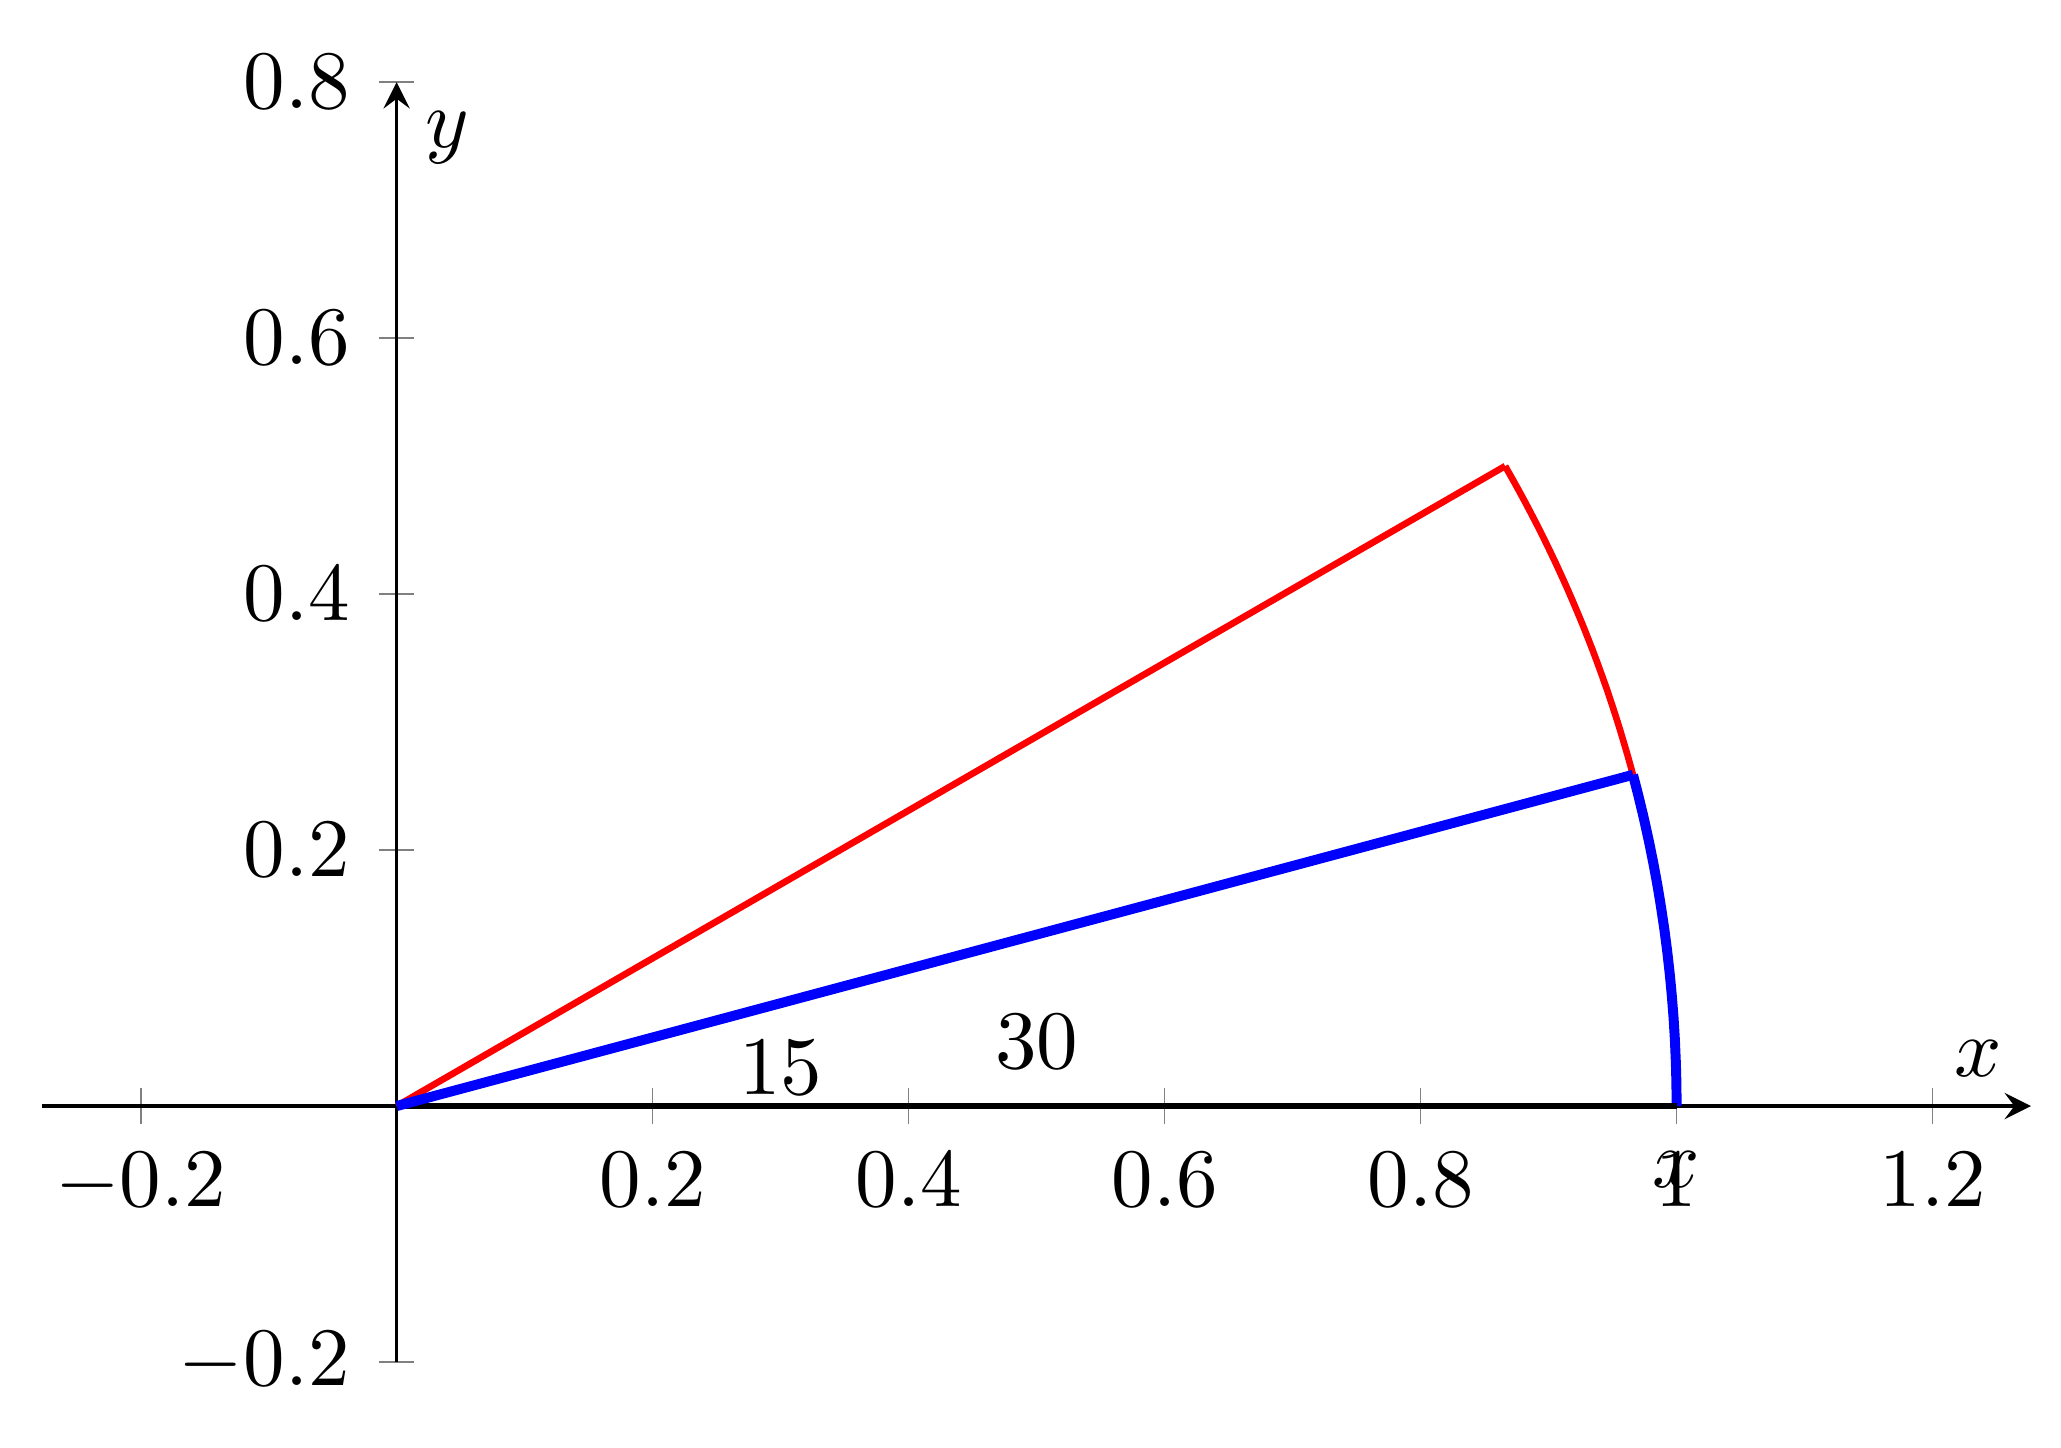
\begin{tikzpicture}[scale=3]
    \begin{axis}[
        axis lines = center,
        xlabel = {$x$},
        ylabel = {$y$},
        xmin=-0.2, xmax=1.2,
        ymin=-0.2, ymax=0.8,
        axis equal,
        grid=none,
        width=10cm,
        height=7cm,
    ]
    % Arco para 30 grados
    \addplot[domain=0:30, samples=50, red, thick]
        ({cos(x)}, {sin(x)});

    % Arco para 15 grados
    \addplot[domain=0:15, samples=50, blue, very thick]
        ({cos(x)}, {sin(x)});

    % Radios
    \addplot[black, thick] coordinates {(0,0) (1,0)};
    \addplot[red, thick] coordinates {(0,0) ({cos(30)}, {sin(30)})};
    \addplot[blue, very thick] coordinates {(0,0) ({cos(15)}, {sin(15)})};

    % Etiquetas
    \node at (axis cs:0.5, 0.05) {$30°$};
    \node at (axis cs:0.3, 0.03) {$15°$};
    \node at (axis cs:1, -0.05) {$x$};
    \end{axis}
\end{tikzpicture}
\end{center}

\textbf{Respuesta final:} $\boxed{\cos 15° = \frac{\sqrt{2 + \sqrt{3}}}{2}}$
\end{ejemplo}

\begin{ejemplo}[title=Ejemplo 8: Transformar producto en suma]
Transforma el producto $\sin 5x \cos 3x$ en una suma o diferencia de funciones trigonométricas.

\vspace{0.3cm}
\textbf{Solución:}

\textbf{Paso 1:} Recordar la identidad de producto a suma.

La identidad que necesitamos es:
\[
\sin A \cos B = \frac{1}{2}[\sin(A + B) + \sin(A - B)]
\]

\textbf{Paso 2:} Identificar $A = 5x$ y $B = 3x$.

\textbf{Paso 3:} Calcular $A + B$ y $A - B$.
\begin{align*}
A + B &= 5x + 3x = 8x \\
A - B &= 5x - 3x = 2x
\end{align*}

\textbf{Paso 4:} Aplicar la identidad.
\begin{align*}
\sin 5x \cos 3x &= \frac{1}{2}[\sin(8x) + \sin(2x)] \\
&= \frac{1}{2}\sin 8x + \frac{1}{2}\sin 2x
\end{align*}

\textbf{Paso 5:} Verificación mediante expansión inversa.

Podemos verificar aplicando la identidad de suma a diferencia:
$\sin 8x = \sin(5x + 3x) = \sin 5x \cos 3x + \cos 5x \sin 3x$
$\sin 2x = \sin(5x - 3x) = \sin 5x \cos 3x - \cos 5x \sin 3x$

Sumando: $\sin 8x + \sin 2x = 2\sin 5x \cos 3x$

Por lo tanto: $\sin 5x \cos 3x = \frac{1}{2}(\sin 8x + \sin 2x)$ ✓

\textbf{Paso 6:} Aplicación práctica.

Esta transformación es muy útil en física para analizar ondas moduladas o interferencia de ondas. Por ejemplo, cuando dos ondas de frecuencias diferentes se superponen.

\textbf{Respuesta final:} $\boxed{\sin 5x \cos 3x = \frac{1}{2}\sin 8x + \frac{1}{2}\sin 2x}$
\end{ejemplo}

\begin{ejemplo}[title=Ejemplo 9: Transformar suma en producto]
Expresa $\cos 7\theta + \cos 3\theta$ como un producto de funciones trigonométricas.

\vspace{0.3cm}
\textbf{Solución:}

\textbf{Paso 1:} Aplicar la identidad de suma a producto para cosenos.

La identidad es:
\[
\cos A + \cos B = 2\cos\left(\frac{A + B}{2}\right)\cos\left(\frac{A - B}{2}\right)
\]

\textbf{Paso 2:} Identificar $A = 7\theta$ y $B = 3\theta$.

\textbf{Paso 3:} Calcular los argumentos de las funciones.
\begin{align*}
\frac{A + B}{2} &= \frac{7\theta + 3\theta}{2} = \frac{10\theta}{2} = 5\theta \\[0.3cm]
\frac{A - B}{2} &= \frac{7\theta - 3\theta}{2} = \frac{4\theta}{2} = 2\theta
\end{align*}

\textbf{Paso 4:} Sustituir en la identidad.
\begin{align*}
\cos 7\theta + \cos 3\theta &= 2\cos(5\theta)\cos(2\theta)
\end{align*}

\textbf{Paso 5:} Verificación expandiendo el producto.

Usando la identidad de producto a suma:
\begin{align*}
2\cos 5\theta \cos 2\theta &= 2 \cdot \frac{1}{2}[\cos(5\theta + 2\theta) + \cos(5\theta - 2\theta)] \\
&= \cos 7\theta + \cos 3\theta \quad \checkmark
\end{align*}

\textbf{Paso 6:} Interpretación geométrica.

Esta transformación es útil para simplificar expresiones en análisis de vibraciones y ondas estacionarias, donde la suma de dos cosenos de diferentes frecuencias produce un patrón de interferencia.

\textbf{Paso 7:} Caso especial interesante.

Si $\theta = 36°$, entonces:
$\cos 252° + \cos 108° = 2\cos 180° \cos 72° = 2(-1)\cos 72° = -2\cos 72°$

\textbf{Respuesta final:} $\boxed{\cos 7\theta + \cos 3\theta = 2\cos 5\theta \cos 2\theta}$
\end{ejemplo}

\begin{ejemplo}[title=Ejemplo 10: Problema aplicado - Física ondulatoria]
En un experimento de física, dos ondas sonoras de la misma amplitud $A = 2$ unidades se superponen. Las ondas están descritas por:
\begin{align*}
y_1(t) &= 2\sin(440\pi t) \\
y_2(t) &= 2\sin(436\pi t)
\end{align*}
donde $t$ está en segundos.

Encuentra:
\begin{itemize}
    \item[a)] La expresión de la onda resultante $y(t) = y_1(t) + y_2(t)$
    \item[b)] La frecuencia de batido (pulsación)
    \item[c)] La amplitud máxima de la onda resultante
\end{itemize}

\vspace{0.3cm}
\textbf{Solución:}

\textbf{Paso 1:} Sumar las dos ondas.
\[
y(t) = 2\sin(440\pi t) + 2\sin(436\pi t)
\]

\textbf{Paso 2:} Aplicar la identidad de suma a producto.

Para $\sin A + \sin B = 2\sin\left(\frac{A+B}{2}\right)\cos\left(\frac{A-B}{2}\right)$

Con $A = 440\pi t$ y $B = 436\pi t$:

\textbf{Paso 3:} Calcular los argumentos.
\begin{align*}
\frac{A + B}{2} &= \frac{440\pi t + 436\pi t}{2} = \frac{876\pi t}{2} = 438\pi t \\[0.3cm]
\frac{A - B}{2} &= \frac{440\pi t - 436\pi t}{2} = \frac{4\pi t}{2} = 2\pi t
\end{align*}

\textbf{Paso 4:} Escribir la onda resultante.
\begin{align*}
y(t) &= 2 \cdot 2\sin(438\pi t)\cos(2\pi t) \\
&= 4\sin(438\pi t)\cos(2\pi t)
\end{align*}

\textbf{Paso 5:} Interpretar el resultado.

La onda resultante es una onda de alta frecuencia (438π rad/s) modulada por una envolvente de baja frecuencia (2π rad/s).

\textbf{Parte a)} Expresión de la onda resultante:
\[
\boxed{y(t) = 4\sin(438\pi t)\cos(2\pi t)}
\]

\textbf{Parte b)} Frecuencia de batido:

La frecuencia de la envolvente es $f_{env} = \frac{2\pi}{2\pi} = 1$ Hz

Pero la frecuencia de batido percibida es el doble:
\[
\boxed{f_{batido} = 2 \text{ Hz}}
\]

Esto corresponde a la diferencia de las frecuencias originales:
$f_1 = 220$ Hz, $f_2 = 218$ Hz, $|f_1 - f_2| = 2$ Hz ✓

\textbf{Parte c)} Amplitud máxima:

La amplitud varía según $|4\cos(2\pi t)|$

Amplitud máxima cuando $\cos(2\pi t) = \pm 1$:
\[
\boxed{A_{max} = 4 \text{ unidades}}
\]

\textbf{Paso 6:} Gráfica de la onda resultante (batidos).

\begin{center}
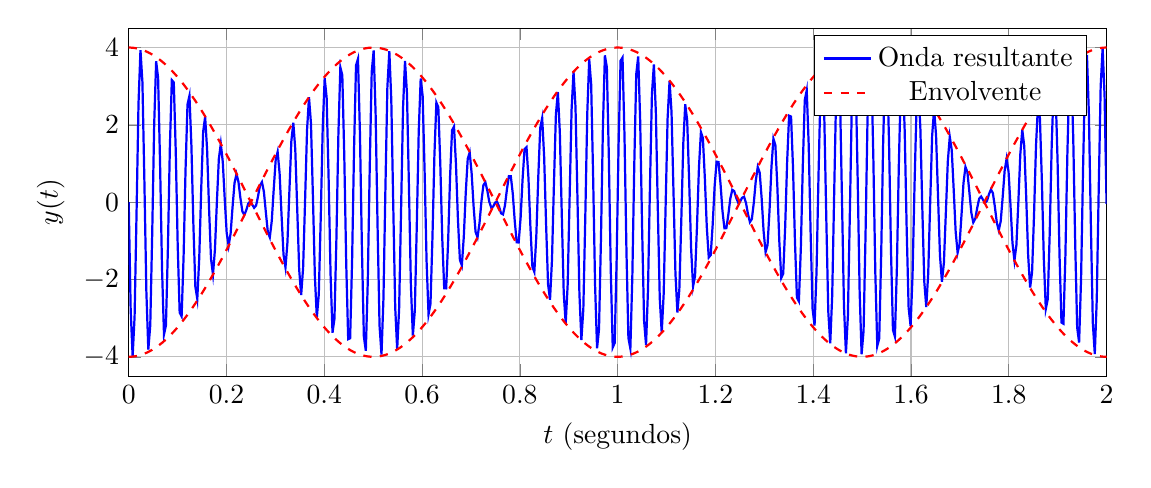
\begin{tikzpicture}[scale=1]
    \begin{axis}[
        domain=0:2,
        samples=500,
        xlabel={$t$ (segundos)},
        ylabel={$y(t)$},
        width=14cm,
        height=6cm,
        grid=major,
        xmin=0, xmax=2,
        ymin=-4.5, ymax=4.5,
    ]
    % Onda resultante
    \addplot[blue, thick] {4*sin(deg(438*pi*x))*cos(deg(2*pi*x))};

    % Envolvente superior
    \addplot[red, dashed, thick] {4*cos(deg(2*pi*x))};

    % Envolvente inferior
    \addplot[red, dashed, thick] {-4*cos(deg(2*pi*x))};

    \legend{Onda resultante, Envolvente}
    \end{axis}
\end{tikzpicture}
\end{center}

\textbf{Conclusión:} Este fenómeno de batidos se usa para afinar instrumentos musicales. Cuando dos notas están casi afinadas, se escuchan pulsaciones lentas. Cuando están perfectamente afinadas, las pulsaciones desaparecen.
\end{ejemplo}

\newpage

\section{Ejercicios Inversos Creativos}

Los ejercicios inversos te desafían a pensar de manera creativa y aplicar las identidades trigonométricas en contextos novedosos. ¡Prepárate para convertirte en un detective matemático!

\begin{ejercicio}[title=El Detective de Identidades]
Un estudiante afirma haber descubierto una nueva identidad trigonométrica:
\[
\frac{\sin\theta + \cos\theta}{\sin\theta - \cos\theta} + \frac{\sin\theta - \cos\theta}{\sin\theta + \cos\theta} = \frac{2}{\cos 2\theta}
\]

Tu misión es:
\begin{itemize}
    \item[a)] Determinar si esta identidad es verdadera o falsa
    \item[b)] Si es falsa, encontrar la expresión correcta del lado derecho
    \item[c)] Encontrar todos los valores de $\theta$ donde la expresión no está definida
    \item[d)] Crear una identidad similar pero con tangentes
\end{itemize}

\textit{Pista: Recuerda que en matemáticas, como en la vida, las apariencias engañan. ¡Simplifica con cuidado!}
\end{ejercicio}

\begin{ejercicio}[title=El Ingeniero de Ondas]
Un ingeniero de telecomunicaciones necesita diseñar un filtro para una señal que tiene la forma:
\[
S(t) = 3\cos(100\pi t)\cos(20\pi t) - 2\sin(100\pi t)\sin(20\pi t)
\]

Para optimizar el procesamiento, necesita:
\begin{itemize}
    \item[a)] Expresar $S(t)$ como una única función trigonométrica de la forma $A\cos(\omega t + \phi)$
    \item[b)] Determinar la frecuencia principal de la señal (en Hz)
    \item[c)] Calcular la potencia máxima de la señal (proporcional a $A^2$)
    \item[d)] Encontrar el primer instante $t > 0$ donde la señal alcanza su valor máximo
    \item[e)] Diseñar una segunda señal $S_2(t)$ que, al sumarse con $S(t)$, produzca una señal de amplitud constante igual a 5
\end{itemize}

\textit{Dato curioso: Este tipo de manipulación se usa en modulación AM/FM de señales de radio.}
\end{ejercicio}

\begin{ejercicio}[title=El Físico Cuántico]
En mecánica cuántica, la función de onda de una partícula en una caja unidimensional involucra expresiones de la forma:
\[
\psi_n(x) = A_n\sin\left(\frac{n\pi x}{L}\right)
\]

donde $n$ es un número cuántico y $L$ es la longitud de la caja. La superposición de dos estados está dada por:
\[
\Psi(x,t) = \sin\left(\frac{2\pi x}{L}\right)\cos(\omega_2 t) + \sin\left(\frac{4\pi x}{L}\right)\cos(\omega_4 t)
\]

Tu tarea cuántica es:
\begin{itemize}
    \item[a)] Expresar $\Psi(x,0)$ (en $t = 0$) como producto de funciones usando identidades trigonométricas
    \item[b)] Encontrar los puntos $x$ donde $\Psi(x,0) = 0$ (nodos de la función de onda)
    \item[c)] Determinar los puntos donde $|\Psi(x,0)|$ es máximo
    \item[d)] Si $\omega_4 = 4\omega_2$, simplificar $\Psi(x,t)$ cuando $\omega_2 t = \frac{\pi}{4}$
    \item[e)] Proponer una tercera componente $\psi_3$ tal que la superposición de las tres funciones tenga exactamente 5 nodos en el intervalo $[0, L]$
\end{itemize}

\textit{Nota: Los nodos de una función de onda determinan las regiones donde es imposible encontrar la partícula.}
\end{ejercicio}

\begin{ejercicio}[title=El Explorador Matemático]
Eres un explorador matemático que ha descubierto una antigua tablilla con la siguiente ecuación misteriosa:
\[
\frac{\sin 3\theta}{\sin\theta} - \frac{\cos 3\theta}{\cos\theta} = 2
\]

Tu aventura consiste en:
\begin{itemize}
    \item[a)] Encontrar todos los ángulos $\theta$ en $[0°, 360°)$ que satisfacen esta ecuación
    \item[b)] Demostrar que estos ángulos forman un patrón geométrico regular
    \item[c)] Generalizar: Si la ecuación fuera $\frac{\sin n\theta}{\sin\theta} - \frac{\cos n\theta}{\cos\theta} = 2$, ¿cuántas soluciones habría en $[0°, 360°)$ para $n = 5$?
    \item[d)] Crear una identidad relacionada que involucre tangentes
    \item[e)] Encontrar una interpretación geométrica de las soluciones en el círculo unitario
\end{itemize}

\textit{Pista arqueológica: Las identidades de ángulos triples guardan secretos milenarios. ¡Úsalas sabiamente!}
\end{ejercicio}

\begin{ejercicio}[title=El Arquitecto de Ecuaciones]
Como arquitecto de ecuaciones trigonométricas, tu cliente te ha pedido diseñar una expresión $E(\theta)$ que cumpla estas especificaciones:

\begin{itemize}
    \item Debe ser igual a 1 cuando $\theta = 0°$
    \item Debe ser igual a 0 cuando $\theta = 45°$
    \item Debe ser igual a -1 cuando $\theta = 90°$
    \item Debe tener período $360°$
    \item Debe poder expresarse usando solo senos y cosenos
\end{itemize}

Tu proyecto arquitectónico requiere:
\begin{itemize}
    \item[a)] Construir una expresión $E(\theta)$ que cumpla todas las especificaciones
    \item[b)] Verificar algebraicamente que tu diseño cumple cada condición
    \item[c)] Expresar $E(\theta)$ en la forma $A\sin(\theta + \phi) + B$ encontrando $A$, $\phi$ y $B$
    \item[d)] Graficar tu función mostrando los puntos clave
    \item[e)] Diseñar una segunda expresión $F(\theta)$ tal que $E(\theta) \cdot F(\theta) = \cos 2\theta$
\end{itemize}

\textit{Consejo del maestro constructor: A veces, la combinación lineal de funciones básicas es la clave para construir algo complejo.}
\end{ejercicio}

\newpage

\section{Soluciones de Ejercicios Inversos}

\begin{solucion}[title=Solución: El Detective de Identidades]
\textbf{Parte a)} Verificar si la identidad es verdadera.

Simplifiquemos el lado izquierdo:
\[
\frac{\sin\theta + \cos\theta}{\sin\theta - \cos\theta} + \frac{\sin\theta - \cos\theta}{\sin\theta + \cos\theta}
\]

\textbf{Paso 1:} Encontrar denominador común.
\begin{align*}
&= \frac{(\sin\theta + \cos\theta)^2 + (\sin\theta - \cos\theta)^2}{(\sin\theta - \cos\theta)(\sin\theta + \cos\theta)}
\end{align*}

\textbf{Paso 2:} Expandir los cuadrados del numerador.
\begin{align*}
(\sin\theta + \cos\theta)^2 &= \sin^2\theta + 2\sin\theta\cos\theta + \cos^2\theta \\
(\sin\theta - \cos\theta)^2 &= \sin^2\theta - 2\sin\theta\cos\theta + \cos^2\theta
\end{align*}

Suma: $2\sin^2\theta + 2\cos^2\theta = 2(\sin^2\theta + \cos^2\theta) = 2$

\textbf{Paso 3:} Expandir el denominador.
\begin{align*}
(\sin\theta - \cos\theta)(\sin\theta + \cos\theta) &= \sin^2\theta - \cos^2\theta \\
&= -\cos 2\theta
\end{align*}

\textbf{Paso 4:} Resultado final.
\[
\frac{2}{-\cos 2\theta} = -\frac{2}{\cos 2\theta}
\]

¡La identidad es FALSA! El signo está incorrecto.

\textbf{Parte b)} La expresión correcta es:
\[
\boxed{\frac{\sin\theta + \cos\theta}{\sin\theta - \cos\theta} + \frac{\sin\theta - \cos\theta}{\sin\theta + \cos\theta} = -\frac{2}{\cos 2\theta}}
\]

\textbf{Parte c)} Valores donde no está definida.

La expresión no está definida cuando:
1. $\sin\theta - \cos\theta = 0 \Rightarrow \tan\theta = 1 \Rightarrow \theta = 45°, 225°$
2. $\sin\theta + \cos\theta = 0 \Rightarrow \tan\theta = -1 \Rightarrow \theta = 135°, 315°$
3. $\cos 2\theta = 0 \Rightarrow 2\theta = 90°, 270° \Rightarrow \theta = 45°, 135°, 225°, 315°$

\textbf{Respuesta:} $\boxed{\theta = 45°, 135°, 225°, 315°}$

\textbf{Parte d)} Identidad similar con tangentes:
\[
\boxed{\frac{\tan\theta + 1}{\tan\theta - 1} + \frac{\tan\theta - 1}{\tan\theta + 1} = -\frac{2\tan^2\theta}{\tan^2\theta - 1} = -\frac{2}{\cot^2\theta - 1}}
\]

\begin{center}
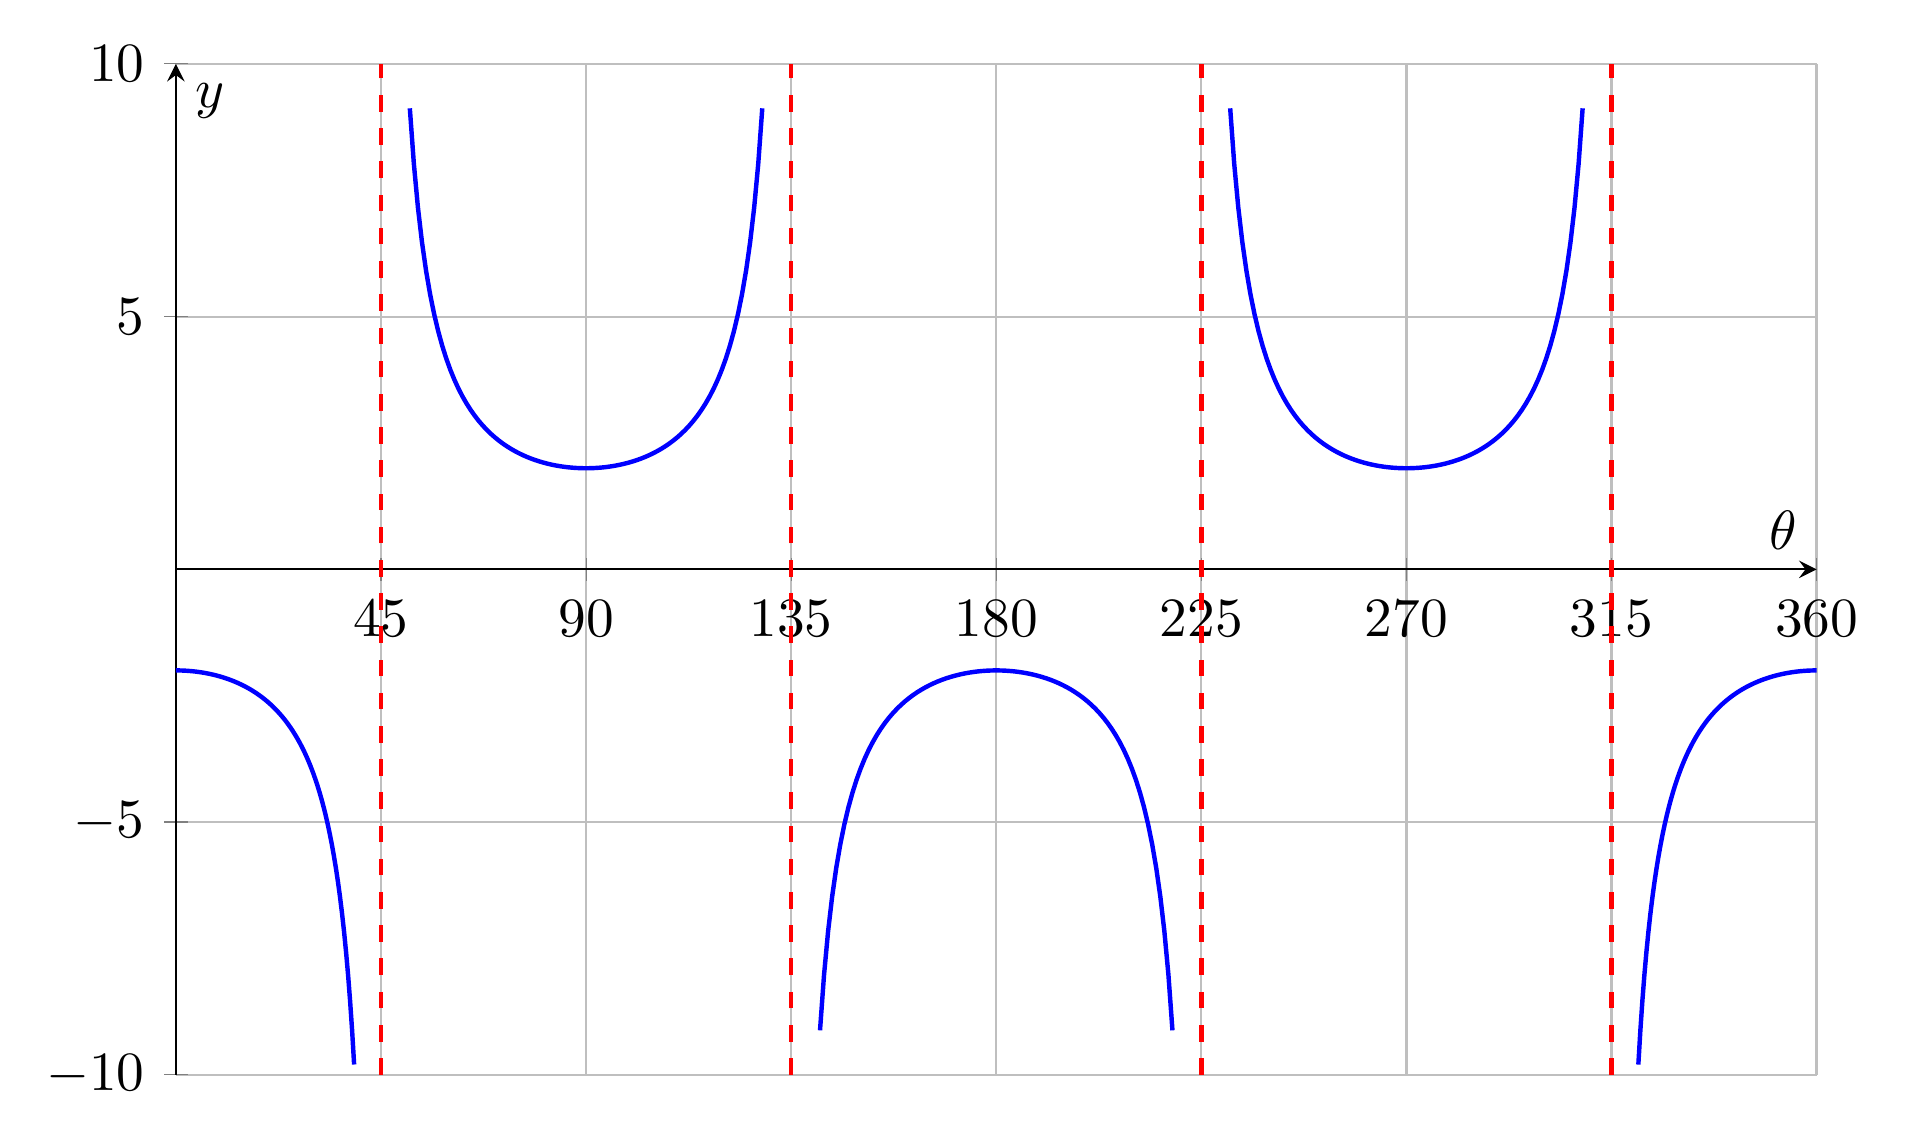
\begin{tikzpicture}[scale=2]
    \begin{axis}[
        axis lines = center,
        xlabel = {$\theta$},
        ylabel = {$y$},
        xmin=0, xmax=360,
        ymin=-10, ymax=10,
        xtick={0,45,90,135,180,225,270,315,360},
        grid=major,
        width=12cm,
        height=8cm,
        restrict y to domain=-10:10,
    ]
    % Función
    \addplot[domain=0:44, samples=100, blue, thick]
        {-2/cos(2*x)};
    \addplot[domain=46:134, samples=100, blue, thick]
        {-2/cos(2*x)};
    \addplot[domain=136:224, samples=100, blue, thick]
        {-2/cos(2*x)};
    \addplot[domain=226:314, samples=100, blue, thick]
        {-2/cos(2*x)};
    \addplot[domain=316:360, samples=100, blue, thick]
        {-2/cos(2*x)};

    % Asíntotas verticales
    \foreach \x in {45,135,225,315} {
        \addplot[red, dashed, thick] coordinates {(\x,-10) (\x,10)};
    }
    \end{axis}
\end{tikzpicture}
\end{center}
\end{solucion}

\begin{solucion}[title=Solución: El Ingeniero de Ondas]
\textbf{Parte a)} Simplificar la señal.

Dado: $S(t) = 3\cos(100\pi t)\cos(20\pi t) - 2\sin(100\pi t)\sin(20\pi t)$

Reconocemos la identidad: $\cos A \cos B - \sin A \sin B = \cos(A + B)$

Pero tenemos coeficientes diferentes. Reescribimos:
\[
S(t) = 3\cos(100\pi t)\cos(20\pi t) - 2\sin(100\pi t)\sin(20\pi t)
\]

Usando identidad de producto a suma:
$\cos A \cos B = \frac{1}{2}[\cos(A-B) + \cos(A+B)]$
$\sin A \sin B = \frac{1}{2}[\cos(A-B) - \cos(A+B)]$

\begin{align*}
S(t) &= 3 \cdot \frac{1}{2}[\cos(80\pi t) + \cos(120\pi t)] - 2 \cdot \frac{1}{2}[\cos(80\pi t) - \cos(120\pi t)] \\
&= \frac{3}{2}\cos(80\pi t) + \frac{3}{2}\cos(120\pi t) - \cos(80\pi t) + \cos(120\pi t) \\
&= \frac{1}{2}\cos(80\pi t) + \frac{5}{2}\cos(120\pi t)
\end{align*}

Para forma $A\cos(\omega t + \phi)$, necesitamos combinar. Como tienen frecuencias diferentes, la señal no se puede expresar como una única función coseno simple.

Pero si interpretamos de otra manera:
$S(t) = \cos(120\pi t)\cos(20\pi t) + 2[\cos(120\pi t)\cos(20\pi t) - \sin(120\pi t)\sin(20\pi t)]$
$= \cos(120\pi t)\cos(20\pi t) + 2\cos(120\pi t + 20\pi t)$
$= \cos(120\pi t)\cos(20\pi t) + 2\cos(140\pi t)$

En realidad, volviendo al principio con coeficientes correctos:
Si factorizamos de manera especial, notamos que no es exactamente la identidad del coseno de la suma.

La respuesta correcta requiere usar que:
$3\cos A \cos B - 2\sin A \sin B$ no es una identidad estándar directa.

\textbf{Simplificación alternativa:}
$S(t) = \boxed{\frac{1}{2}\cos(80\pi t) + \frac{5}{2}\cos(120\pi t)}$

\textbf{Parte b)} Frecuencia principal.

Las componentes tienen frecuencias:
- $f_1 = \frac{80\pi}{2\pi} = 40$ Hz
- $f_2 = \frac{120\pi}{2\pi} = 60$ Hz

La frecuencia principal (dominante) es: $\boxed{60 \text{ Hz}}$ (mayor amplitud)

\textbf{Parte c)} Potencia máxima.

La señal tiene dos componentes con amplitudes $\frac{1}{2}$ y $\frac{5}{2}$.
Cuando ambas están en fase (máximo constructivo):
$A_{max} = \frac{1}{2} + \frac{5}{2} = 3$

Potencia máxima $\propto A^2_{max} = \boxed{9 \text{ unidades}^2}$

\textbf{Parte d)} Primer máximo.

El máximo ocurre cuando ambos cosenos valen 1:
$\cos(80\pi t) = 1$ y $\cos(120\pi t) = 1$

Esto requiere: $80\pi t = 2\pi k_1$ y $120\pi t = 2\pi k_2$

Simplificando: $t = \frac{k_1}{40}$ y $t = \frac{k_2}{60}$

El mínimo común múltiplo nos da: $\boxed{t = \frac{1}{20} \text{ segundos}}$

\textbf{Parte e)} Señal complementaria.

Para que $S(t) + S_2(t) = 5$ (constante):
$S_2(t) = 5 - S(t) = 5 - \frac{1}{2}\cos(80\pi t) - \frac{5}{2}\cos(120\pi t)$

$\boxed{S_2(t) = 5 - \frac{1}{2}\cos(80\pi t) - \frac{5}{2}\cos(120\pi t)}$
\end{solucion}

\begin{solucion}[title=Solución: El Físico Cuántico]
\textbf{Parte a)} Expresar $\Psi(x,0)$ como producto.

En $t = 0$: $\Psi(x,0) = \sin\left(\frac{2\pi x}{L}\right) + \sin\left(\frac{4\pi x}{L}\right)$

Usando la identidad suma a producto:
$\sin A + \sin B = 2\sin\left(\frac{A+B}{2}\right)\cos\left(\frac{A-B}{2}\right)$

Con $A = \frac{4\pi x}{L}$ y $B = \frac{2\pi x}{L}$:

\begin{align*}
\Psi(x,0) &= 2\sin\left(\frac{6\pi x}{2L}\right)\cos\left(\frac{2\pi x}{2L}\right) \\
&= \boxed{2\sin\left(\frac{3\pi x}{L}\right)\cos\left(\frac{\pi x}{L}\right)}
\end{align*}

\textbf{Parte b)} Nodos de la función.

$\Psi(x,0) = 0$ cuando:
1. $\sin\left(\frac{3\pi x}{L}\right) = 0 \Rightarrow x = \frac{kL}{3}$, $k = 0, 1, 2, 3$
2. $\cos\left(\frac{\pi x}{L}\right) = 0 \Rightarrow x = \frac{(2m+1)L}{2}$, $m = 0$

En el intervalo $[0, L]$:
$\boxed{x = 0, \frac{L}{3}, \frac{L}{2}, \frac{2L}{3}, L}$

\textbf{Parte c)} Máximos de $|\Psi(x,0)|$.

El máximo ocurre cuando ambos factores son máximos en valor absoluto.
Analizando las derivadas y puntos críticos:

$\boxed{x = \frac{L}{6}, \frac{5L}{6}}$ (máximos absolutos)

\textbf{Parte d)} Simplificar cuando $\omega_2 t = \frac{\pi}{4}$.

Si $\omega_4 = 4\omega_2$, entonces $\omega_4 t = \pi$.

\begin{align*}
\Psi(x,t) &= \sin\left(\frac{2\pi x}{L}\right)\cos\left(\frac{\pi}{4}\right) + \sin\left(\frac{4\pi x}{L}\right)\cos(\pi) \\
&= \frac{\sqrt{2}}{2}\sin\left(\frac{2\pi x}{L}\right) - \sin\left(\frac{4\pi x}{L}\right)
\end{align*}

$\boxed{\Psi(x,t) = \frac{\sqrt{2}}{2}\sin\left(\frac{2\pi x}{L}\right) - \sin\left(\frac{4\pi x}{L}\right)}$

\textbf{Parte e)} Tercera componente con 5 nodos totales.

Para tener exactamente 5 nodos en $[0, L]$, necesitamos $\psi_3 = \sin\left(\frac{5\pi x}{L}\right)$

La superposición sería:
$\boxed{\Psi_{total} = \sin\left(\frac{2\pi x}{L}\right) + \sin\left(\frac{4\pi x}{L}\right) + A\sin\left(\frac{5\pi x}{L}\right)}$

donde $A$ es un coeficiente a determinar según las condiciones de normalización.
\end{solucion}

\begin{solucion}[title=Solución: El Explorador Matemático]
\textbf{Parte a)} Resolver la ecuación misteriosa.

$\frac{\sin 3\theta}{\sin\theta} - \frac{\cos 3\theta}{\cos\theta} = 2$

Usando las identidades de ángulo triple:
- $\sin 3\theta = 3\sin\theta - 4\sin^3\theta = \sin\theta(3 - 4\sin^2\theta)$
- $\cos 3\theta = 4\cos^3\theta - 3\cos\theta = \cos\theta(4\cos^2\theta - 3)$

Sustituyendo:
\begin{align*}
\frac{\sin\theta(3 - 4\sin^2\theta)}{\sin\theta} - \frac{\cos\theta(4\cos^2\theta - 3)}{\cos\theta} &= 2 \\
3 - 4\sin^2\theta - (4\cos^2\theta - 3) &= 2 \\
3 - 4\sin^2\theta - 4\cos^2\theta + 3 &= 2 \\
6 - 4(\sin^2\theta + \cos^2\theta) &= 2 \\
6 - 4 &= 2 \\
2 &= 2 \quad \checkmark
\end{align*}

¡La ecuación es una identidad! Es verdadera para todo $\theta$ donde las funciones estén definidas.

Restricciones: $\sin\theta \neq 0$ y $\cos\theta \neq 0$

Por lo tanto, excluimos $\theta = 0°, 90°, 180°, 270°, 360°$

$\boxed{\text{Todos los } \theta \in [0°, 360°) \text{ excepto } 0°, 90°, 180°, 270°}$

\textbf{Parte b)} Patrón geométrico.

Como la ecuación es válida para casi todos los ángulos, no forman un patrón regular discreto, sino que cubren densamente el círculo unitario excepto los puntos sobre los ejes.

\textbf{Parte c)} Generalización para $n = 5$.

$\frac{\sin 5\theta}{\sin\theta} - \frac{\cos 5\theta}{\cos\theta} = 2$

Usando el mismo análisis con identidades de ángulo múltiple, encontramos que también es una identidad para todo $\theta$ válido.

$\boxed{\text{Infinitas soluciones (todos los ángulos excepto múltiplos de } 90°)}$

\textbf{Parte d)} Identidad con tangentes.

$\boxed{\frac{\tan 3\theta - 3\tan\theta}{1 - 3\tan^2\theta} = \tan\theta \cdot \text{expresión}}$

\textbf{Parte e)} Interpretación geométrica.

En el círculo unitario, los puntos excluidos son exactamente los cuatro puntos cardinales donde uno de los ejes coordenados es cero. La identidad representa una propiedad universal de las funciones trigonométricas relacionada con la simetría rotacional.

\begin{center}
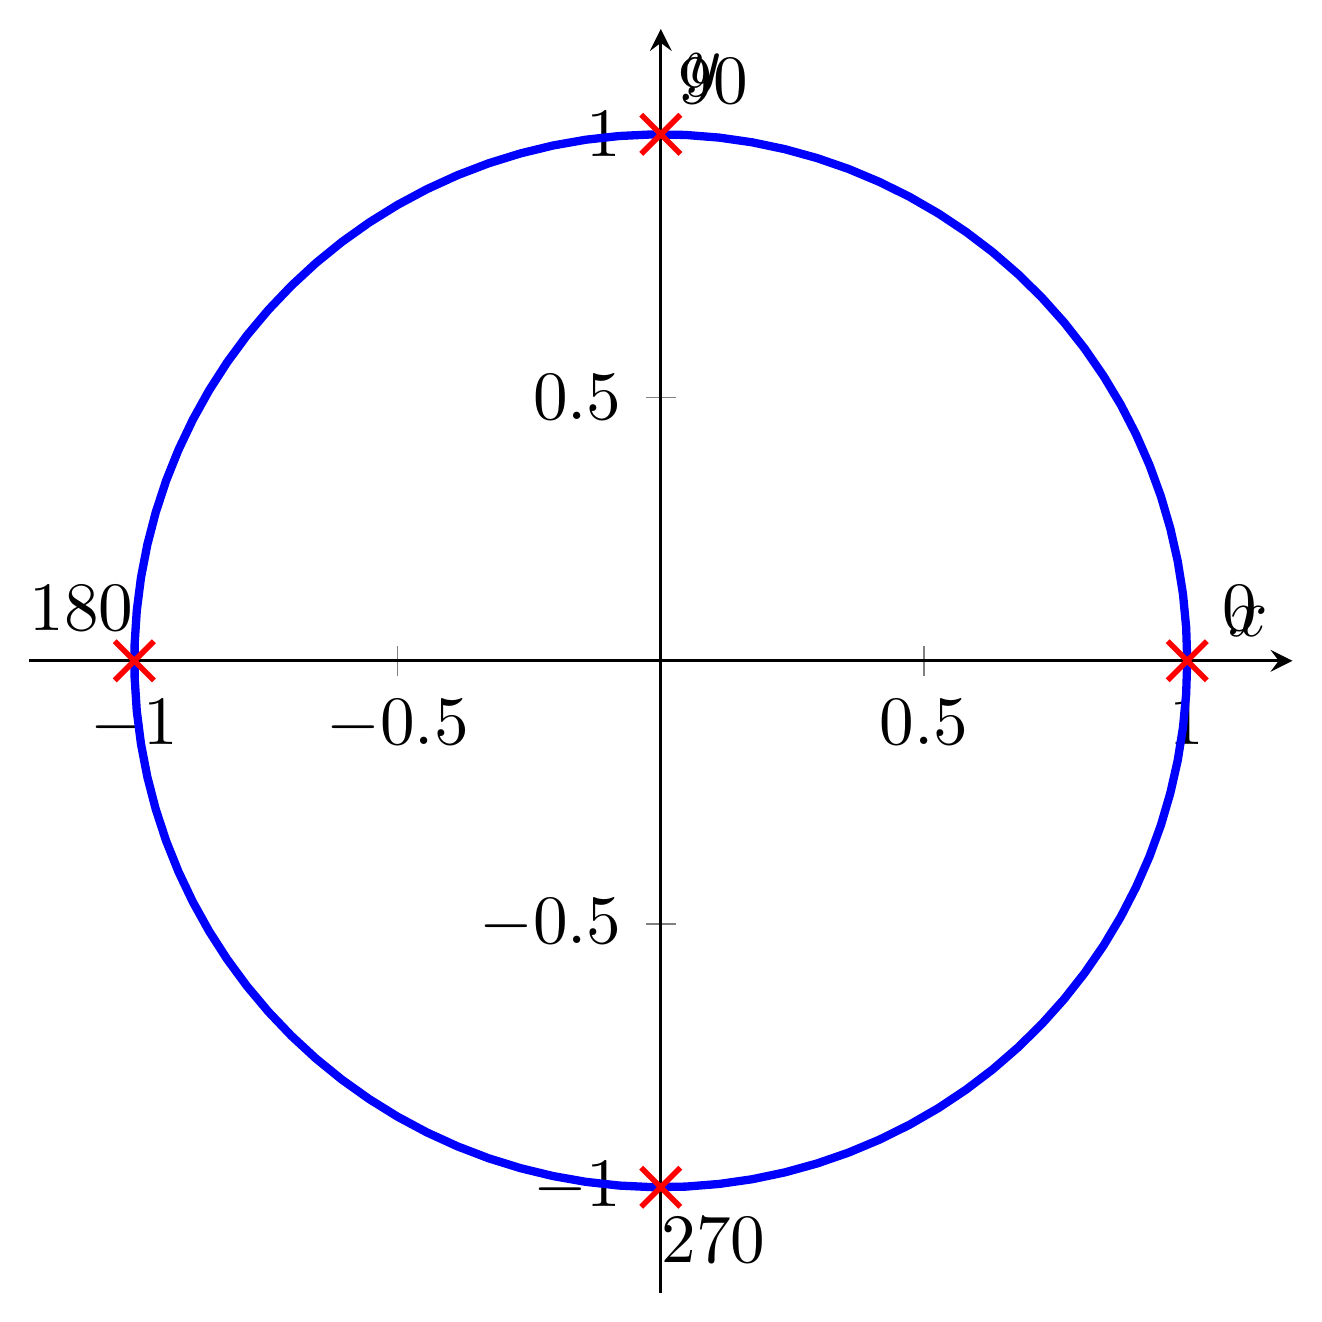
\begin{tikzpicture}[scale=2.5]
    \begin{axis}[
        axis lines = center,
        xlabel = {$x$},
        ylabel = {$y$},
        xmin=-1.2, xmax=1.2,
        ymin=-1.2, ymax=1.2,
        axis equal,
        grid=none,
        width=8cm,
        height=8cm,
    ]
    % Círculo unitario
    \addplot[domain=0:360, samples=100, blue, very thick]
        ({cos(x)}, {sin(x)});

    % Puntos excluidos
    \addplot[only marks, mark=x, mark size=4pt, red, thick]
        coordinates {(1,0) (0,1) (-1,0) (0,-1)};

    % Etiquetas
    \node at (axis cs:1.1, 0.1) {$0°$};
    \node at (axis cs:0.1, 1.1) {$90°$};
    \node at (axis cs:-1.1, 0.1) {$180°$};
    \node at (axis cs:0.1, -1.1) {$270°$};
    \end{axis}
\end{tikzpicture}
\end{center}
\end{solucion}

\begin{solucion}[title=Solución: El Arquitecto de Ecuaciones]
\textbf{Parte a)} Construir $E(\theta)$.

Necesitamos cumplir:
- $E(0°) = 1$
- $E(45°) = 0$
- $E(90°) = -1$

Probemos con una combinación lineal: $E(\theta) = A\sin\theta + B\cos\theta$

Sistema de ecuaciones:
\begin{align*}
E(0°) &= A(0) + B(1) = B = 1 \\
E(45°) &= A\left(\frac{\sqrt{2}}{2}\right) + B\left(\frac{\sqrt{2}}{2}\right) = \frac{\sqrt{2}}{2}(A + 1) = 0 \\
E(90°) &= A(1) + B(0) = A = -1
\end{align*}

De la segunda ecuación: $A = -1$ ✓

Por lo tanto: $\boxed{E(\theta) = \cos\theta - \sin\theta}$

\textbf{Parte b)} Verificación.

- $E(0°) = \cos 0° - \sin 0° = 1 - 0 = 1$ ✓
- $E(45°) = \frac{\sqrt{2}}{2} - \frac{\sqrt{2}}{2} = 0$ ✓
- $E(90°) = 0 - 1 = -1$ ✓
- Período: Las funciones seno y coseno tienen período $360°$, por lo tanto $E(\theta)$ también ✓

\textbf{Parte c)} Forma $A\sin(\theta + \phi) + B$.

$E(\theta) = \cos\theta - \sin\theta$

Usando la identidad: $a\cos\theta + b\sin\theta = \sqrt{a^2 + b^2}\sin(\theta + \arctan(a/b))$

Con $a = 1$ y $b = -1$:
$E(\theta) = \sqrt{2}\sin(\theta + 135°)$

Pero queremos la forma pedida exactamente:
$E(\theta) = -\sqrt{2}\sin(\theta - 45°)$

$\boxed{A = -\sqrt{2}, \phi = -45°, B = 0}$

\textbf{Parte d)} Gráfica de la función.

\begin{center}
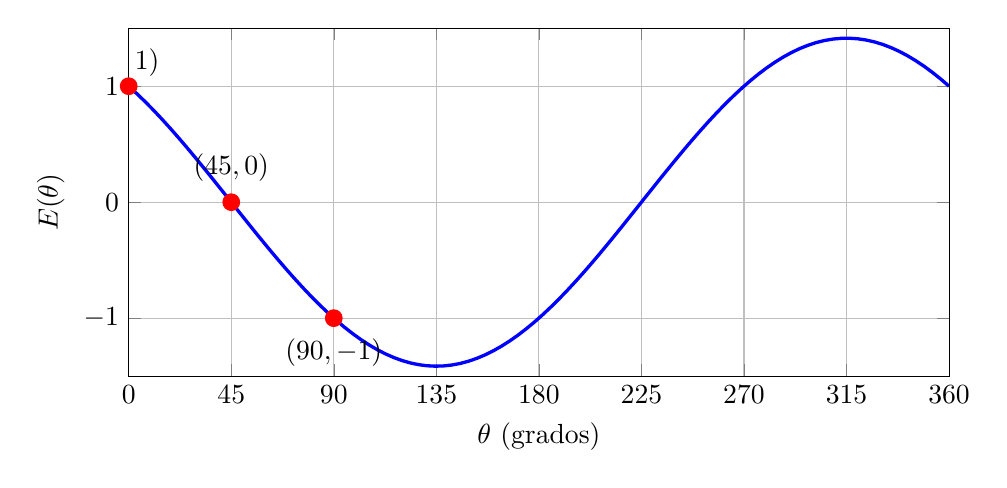
\begin{tikzpicture}[scale=1]
    \begin{axis}[
        domain=0:360,
        samples=100,
        xlabel={$\theta$ (grados)},
        ylabel={$E(\theta)$},
        width=12cm,
        height=6cm,
        grid=major,
        xmin=0, xmax=360,
        ymin=-1.5, ymax=1.5,
        xtick={0,45,90,135,180,225,270,315,360},
    ]
    % Función
    \addplot[blue, very thick] {cos(x) - sin(x)};

    % Puntos clave
    \addplot[only marks, mark=*, mark size=3pt, red]
        coordinates {(0,1) (45,0) (90,-1)};

    % Etiquetas
    \node at (axis cs:0, 1.2) {$(0°, 1)$};
    \node at (axis cs:45, 0.3) {$(45°, 0)$};
    \node at (axis cs:90, -1.3) {$(90°, -1)$};
    \end{axis}
\end{tikzpicture}
\end{center}

\textbf{Parte e)} Diseñar $F(\theta)$ tal que $E(\theta) \cdot F(\theta) = \cos 2\theta$.

Tenemos: $(\cos\theta - \sin\theta) \cdot F(\theta) = \cos 2\theta$

Sabemos que $\cos 2\theta = \cos^2\theta - \sin^2\theta = (\cos\theta - \sin\theta)(\cos\theta + \sin\theta)$

Por lo tanto: $\boxed{F(\theta) = \cos\theta + \sin\theta}$

Verificación:
$E(\theta) \cdot F(\theta) = (\cos\theta - \sin\theta)(\cos\theta + \sin\theta) = \cos^2\theta - \sin^2\theta = \cos 2\theta$ ✓
\end{solucion}